\documentclass[a4paper,12pt]{article}
\usepackage{cmap}
\usepackage[utf8]{inputenc}
\usepackage[warn]{mathtext}
\usepackage{epsf,amsmath,amsfonts,amssymb,amsbsy}
\usepackage[mathscr]{eucal}
\usepackage[english, russian]{babel}
\usepackage[left=1cm,right=2cm,top=2cm,bottom=2cm]{geometry}
\usepackage{graphicx}
\usepackage{indentfirst}
\DeclareGraphicsExtensions{.pdf,.png,.jpg}
\usepackage{pgfplots}
\begin{document}

\section{Аннотация}
В этой работе были исследованы классические методы автоматической бинаризации изображений. Была написана программа, демонстрирующая работу популярных методов глобальной и адаптивной бинаризации. Также был сделан веб-сайт, чтобы каждый мог самостоятельно бинаризовать изображения в пару кликов.
\section{Описание различных методов бинаризации}
Главной целью бинаризации является радикальное уменьшение количества информации, с которой приходится работать. Удачная бинаризация сильно упрощает последующую работу с
изображением.

\begin{figure}[h!]
    \centering	
    \includegraphics[width=1.05\textwidth]{bin.png}
    \label{1_1}
\end{figure}

Существуют различные методы бинаризации, которые можно условно разделить на две
группы:

- глобальные (пороговые);

- локальные (адаптивные).
\subsection{Глобальные методы бинаризации}
В глобальных методах бинаризации происходит работа со всем изображением сразу. В ходе работы находится порог бинаризации $t$, с помощью которого происходит деление на черное и белое, причем величина порога $t$ остается неизменной в течение всего процесса бинаризации.



\subsubsection*{Метод Оцу}

Популярным методом глобальной бинаризации изображений является метод Оцу.

С помощью данного метода вычисляется порог $t$, минимизирующий среднюю ошибку сегментации, т.е. среднюю ошибку от принятия решения о принадлежности пикселей
изображения объекту или фону. Значения яркостей пикселей изображения можно рассматривать как случайные величины, а их гистограмму – как оценку плотности распределения вероятностей. Если плотности распределения вероятностей известны, то можно определить оптимальный (в смысле минимума ошибки) порог для сегментации изображения на
два класса c0 и c1 (объекты и фон).

Гистограмма строится по значениям $p_i = \frac{ni}{N}$. В данной формуле N – общее количество пикселей изображения с уровнем яркости i. Порог t представляет собой целое значение от 0 до L=max. При помощи гистограммы все пиксели разделяются на «полезные» (объектные») и фоновые. Каждому виду соответствуют относительные частоты $W_0$ и $W_1$:

\begin{equation}
    W_0(t) = \sum_{i=1}^t p_i
\end{equation}

\begin{equation}
    W_1(t) = \sum_{i=t+1}^L p_i = 1 - W_0(t)
\end{equation}

Далее вычисляются средние уровни для каждого вида изображения по формулам:
\begin{equation}
    \mu_0(t) = \sum_{i=1}^t \frac{i p_i}{W_0}
\end{equation}

\begin{equation}
    \mu_1(t) = \sum_{i=t+1}^L \frac{i p_i}{W_1}
\end{equation}

Далее ищется порог, который уменьшает дисперсию внутри вида пикселей, определяемую
следующей формулой:
\begin{equation}
    \delta_W^2(t) = W_1(t)\delta_1^2(t) + W_2(t)\delta_2^2(t)
\end{equation}

Следующим шагом определяется межклассовая дисперсия, по формуле, представленной
ниже:
\begin{equation}
    \sigma_{\text{кл}}^2(t) = W_0(t)W_1(t) * (\mu_1(t) - \mu_0(t))^2
\end{equation}

Затем вычисляется максимальное значение для оценки качества деления изображения на
две части, которое соответствует искомому порогу:
\begin{equation}
    \eta(t) = max \left[\frac{\sigma_{\text{кл}}^2(t)}{\delta_W^2(t)}\right]
\end{equation}
Достоинствами метода Оцу являются:

- простота реализации;

- адаптация к различного рода изображениям, при помощи выбора оптимального порога;

- быстрое время выполнения.

\subsubsection*{ISODATA}
Алгоритм ISODATA является разновидностью итерационных
алгоритмов, в основе которого лежит метод разделения-объединения
кластеров.

Алгоритм формирования кластеров строится следующим образом.
Имеется множество кластеров $C_1$, $C_2$, …, $C_k$ с математическими
ожиданиями $m_1$, $m_2$, …, $m_k$ и ковариационная матрица $\sum_{k}$ для $k$-го кластера. 

Шаги алгоритма:

1. Поместить вектор $x_i$ в кластер $l$, для которого достигается
минимум
\begin{equation*}
    D_M = (x_i - m_l)^\prime {\sum_{l}}^{-1}(x_l - m_l)
\end{equation*}

2. Объединить кластеры $i$ и $j$, если
\begin{equation*}
    |m_i - m_j| < \tau_\nu
\end{equation*}
где $\tau_\nu$ – пороговое значение дисперсии.

3. Разделить кластер $k$, если максимальное собственное значение $\sum_{k}$ превышает порог $\tau_\nu$.

4. Завершить работу, если для каждого кластера $I$ выполняется
условие 
\begin{equation*}
    |m_i(t) - m_i(t+1)| < \varepsilon 
\end{equation*}
или если достигнуто максимально допустимое значение итераций.
\vspace{1,5cm}
\subsection{Локальные методы бинаризации}

Локальные (адаптивные) методы бинаризации производят разбивку изображение на
несколько областей, для каждой из которых необходимо вычислить порог, основываясь на
информации об интенсивности пикселей.

Алгоритмы данного класса предполагают разбиение изображения на блоки определенного
размера, при этом размер блока должен быть минимальным, но достаточным для сохранения
исходных особенностей и деталей изображения. Однако при этом блоки должны быть
настолько большими, чтобы шумы влияли на результат минимально. Функция сглаживания результирующего растра при адаптивной бинаризации позволяет получить
удовлетворительный результат без использования дополнительных фильтров.

\subsubsection*{Метод Ниблэка}
В методе Ниблэка для каждого пикселя изображения необходимо получить свое значение
порога. Его величина определяется на основе вычисления локального среднего и локального
среднеквадратического отклонения. Значение порога для точки с координатами (m, n)
считается по следующей формуле:
\begin{equation}
    t(m,n) = \mu(m,n) + k*\sigma(m,n)
\end{equation}

В данной формуле $\mu (m,n)$ представляет собой среднее, $\sigma (m, n)$ – среднеквадратичное
отклонение в локальной окрестности рассматриваемой точки изображения, а значение $k$
определяет, какую именно часть границы объекта необходимо взять в качестве объекта.
Метод Ниблэка за счет своей простоты позволяет достичь наиболее высокую скорость
бинаризации изображений. Метод используется на практике для быстрой фильтрации
контрастных изображений, на которых практически отсутствуют сильно зашумленные участки
с плавными переходами яркости.

\subsubsection*{Метод Саувола}
К методам локальной адаптивной бинаризации относится и метод Саувола. Определение
локального порога бинаризации осуществляется с помощью прохождения всего изображения
окном w w. В методе бинаризации Саувола порог $t(x,y)$ определяется следующей формулой,
используя для вычисления среднее значения $m(x, y)$ и среднеквадратическое отклонение $s(x, y)$
интенсивности пиксела в окне w w вокруг пиксела $(x, y)$:
\begin{equation}
    t(x,y) = m(x,y)\left[1 + k\left(\frac{s(x,y)}{R} - 1\right)\right]
\end{equation}
В данной формуле $R$ представляет максимальное отклонение ($R$ = 128 для изображения в
оттенках серого), а $k$ является параметром, который принимает значения в диапазоне [0.2, 0.5].

Метод Саувола широко применяется к изображениям, в которых яркость изображения
распределяется неравномерно. Однако, алгоритм Саувола менее устойчив к зашумленности
исходного изображения, чем, к примеру, алгоритм Оцу. Также у метода имеются трудности с
изображениями, у которых мало освещения, особенно в случаях, когда значения пикселей
объекта находятся близко друг к другу. При обработке тонких пересекающихся линий могут
возникать разрывы, поэтому метод хорош для толстых линий и крупных объектов.
\vspace{1.3cm}

В общем случае адаптивную бинаризацию можно рекомендовать в случае, если необходимо
обработать для обработки полутоновых изображений невысокого качества (сканированных снимок),
на которых из-за неравномерности фона обычная бинаризация дает плохие результаты. 

\section{Реализация программы для демонстрации методов}

Для демонстрации работы написанной программы, мы собрали DataSet из разнообразных фотографий и пропустили их через наш код. Полученные результаты исполнения можно наблюдать ниже.

\subsection*{Скан текста}

Для начала был набран, распечатан и отсканирован текст. Его скан мы подали реализованным методам нашей программы. Как можно видеть из изображения ниже, все методы, за исключением Niblack, хорошо справились с поставленной задачей бинаризации скана распечатанного текста. Полученный результат можно объяснить ограниченной областью примения метода Niblack.
\begin{figure}[h!]
    \centering	
    \includegraphics[width=1.05\textwidth]{1.jpg}
    \label{1_1}
\end{figure}
\newpage
\subsection*{Скан текста c дефектами}

Далее нам стало интересно, как данные методы бинаризации изображения справляются с различными дефектами на фотографии. Для этого мы разлили чай на листок с текстом и скомкали его, а потом отсканировали ещё раз. Как можно наблюдать из результатов применения методов, адаптивные справились с бинаризацией хуже из-за шумов. Так же можно заметить, что дефекты на скане практически никак не отобразились на работе глобальных методов. 
\begin{figure}[h!]
    \centering	
    \includegraphics[width=0.95\textwidth]{2.jpg}
    \label{1_1}
\end{figure}

\subsection*{DIBCO 2016}
DIBCO - самый популярный конкурс по бинаризации рукописного и печатного текста. Мы решили посмотреть, как данные методы справятся с фотографией, предложенной на одном из соревнований. Оснавная сложность оригинального изображения заключается в просвечевании текста с другой стороны листа. Методы Оцу и Isodata отлично справились с этим. А вот результаты применения адаптивных методов, особенно Niblack, имеют на своём фоне большое количество шумов, мешающее нормальному распознованию текста.  
\begin{figure}[h!]
    \centering	
    \includegraphics[width=0.95\textwidth]{3.jpg}
    \label{1_1}
\end{figure}

\subsection*{Текст с неоднородной яркостью фона}
Слабым местом пороговых методов является неоднородная яркость фона. Это можно пронаблюдать на изображении ниже. В области тени, после применения методов Оцу и Isodata, возникает тёмное пятно. Адаптивные же методы хорошо справляются с этой задачей, так как они работают с окнами.
\begin{figure}[h!]
    \centering	
    \includegraphics[width=0.95\textwidth]{4.jpg}
    \label{1_1}
\end{figure}

\subsection*{Медицинсике изображения}
Также нам было интересно посмотреть, как хорошо данные методы справляются с бинаризацией медицинских изображений. Так как на таких фотографиях обычно большое количество шумов, то для  них желательно использовать пороговые методы. А лучший результат даёт метод Оцу. Изображения ниже, с применением данных методов для медицинский фотографий, подтверждают выше сказанное.
\begin{figure}[h!]\centering
\begin{tabular}{cc}
\includegraphics[width=0.5\textwidth]{5.jpg}
&
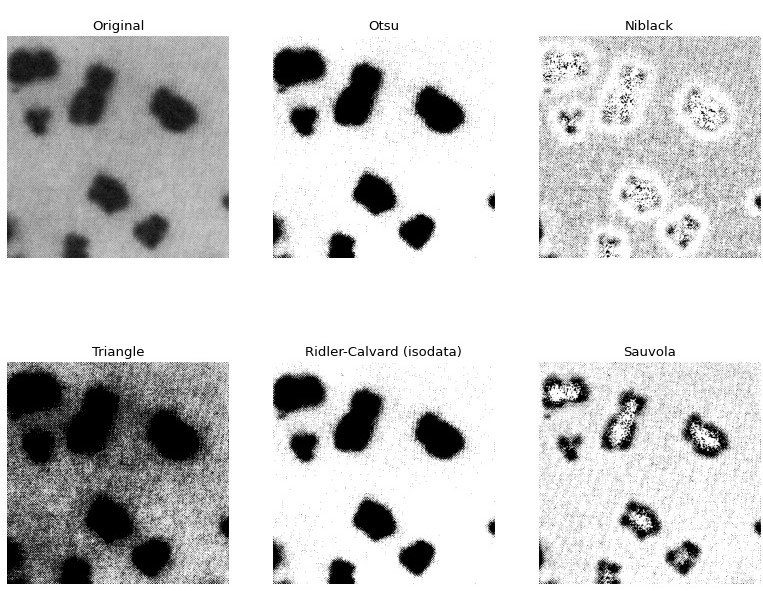
\includegraphics[width=0.54\textwidth]{6.jpg}
\end{tabular}
\end{figure}

\section{Вывод}
Неудачи в процессе бинаризации могут привести к искажениям, таким, как разрывы в
линиях, потеря значащих деталей, нарушение целостности объектов, появление шума и
непредсказуемое искажение символов из-за неоднородностей фона.

Различные методы бинаризации имеют свои слабые места: так, например, метод Оцу может
приводить к утрате мелких деталей и «слипанию» близлежащих символов, а метод Ниблэка
грешит появлением ложных объектов в случае неоднородностей фона с низкой
контрастностью. Из этого можно сделать вывод, что каждый из рассмотренных методов должен
быть применен в определенной области, а также для каждой области могут быть разработаны
более подходящие методы.
\newpage
\begin{center}
    \subsubsection*{{Список литературы/References}}
\end{center}

\begin{enumerate}
    \item \textit{Исрафилов Х.С.} Исследование методов бинаризации изображений.
    \item \textit{N. Otsu.} A threshold selection method from gray-level histograms (англ.) // IEEE Trans. Sys., Man., Cyber. : journal. — 1979. — Vol. 9. — P. 62—66
    \item \textit{Селянкин В.В, Скороход С.В.} Анализ и обработка изображений в задачах компьютерного зрения - с.65-66
    \item Сегментация изображения. [Электронный ресурс] https://habr.com/ru/post/128768/
\end{enumerate}
\end{document}
